\chapter{面向异质数据的隐私保护梯度聚合技术}

\section{引言}
联邦学习\cite{mcmahan2017communication}(FL)是由Google在2017年提出的一种新颖的分布式机器学习框架,适用于注重数据隐私的参与方在服务器的调动下,协同完成神经网络的训练。
在工业界,目前已经有很多基于联邦学习的实际应用已经完成落地,Google基于联邦学习为移动端打造的智能输入法预测方案 \cite{hard2018federated},医疗行业基于联邦学习落地的智能诊断和治疗系统 \cite{li2020deepfed},以及微众银行基于联邦学习的构建的风险评估系统 \cite{DBLP:conf/ndss/CaoF0G21}。 
简单来说,FL的核心步骤,是在FL服务提供商的协调下,不同的参与方上传本地训练得到的本地更新(即梯度),然后由服务提供商聚合梯度生成全局模型,最后分发给参与方。在整个过程中,用户的数据始终保持在本地,对比传统的分布式机器学习直接交易数据的方式,提升了数据的隐私性。

然而,一些研究 \cite{geiping2020inverting,zhu2019deep,gao2021privacy} 表明,尽管没有直接上传数据,但是FL仍然存在隐私泄露的风险,服务提供商可以通过用户上传的梯度推断出用户的原始数据集,这违背了一些数据保护法,比如GDPR。
同时也有研究 \cite{zhao2018federated, tuor2021overcoming, yoshida2019hybrid}表明,异质数据(即用户间数据分布不一致)给FL的联合训练准确率带来了较大的挑战。
具体来说,真实场景下的FL,往往会遇到参与方数据分布不一致的情况,这会导致参与方的局部目标函数和全局的目标函数之间出现偏差,从而大大影响经典FL训练得到的全局模型的性能。

%TODO 加一个 权重偏差的图

为了解决FL中的梯度隐私泄露问题,许多基于密码协议的安全聚合方案 \cite{liu2021privacy, aono2017privacy, zhang2020batchcrypt, dong2021flod, hao2021efficient} 被学者们提出来。
比如说,一些方案 \cite{liu2021privacy, aono2017privacy, zhang2020batchcrypt} 使用同态加密(HE)来对用户梯度加密,而服务提供商需要在密文状态下进行梯度的聚合,所以能够很好的保护用户梯度的隐私。
除此之外,一些方案 \cite{hao2021efficient, dong2021flod} 利用安全多方计算技术(MPC)来实现梯度的隐私保护,可以在不泄漏用户梯度的情况下,完成梯度的聚合。
在另一方面,为了解决异质数据带来的挑战,一些方案 \cite{li2020federated, gao2022feddc, ghosh2020efficient, briggs2020federated}对经典的FL平均聚合方法(FedAvg\cite{mcmahan2017communication})做了改良,比如说,方案 \cite{li2020federated} 对用户本地训练过程进行了微调,在本地目标函数中添加了一个正则项,用来限制不同用户梯度之间的偏差。

尽管许多工作都在致力于解决FL中的梯度隐私泄露问题,以及数据异质问题,但是他们往往将两个问题分开讨论。
许多解决梯度隐私泄露问题的工作,都没有考虑到异质数据对FL发起的挑战,在面对异质数据时,性能表现地下。而许多提升异质数据联合训练性能的方案,都没有考虑到梯度的隐私泄露问题,直接使用梯度明文进行聚合。其中文献 \cite{xiong2021privacy} 基于差分隐私(DP)同时考虑了上述两个问题,但是对梯度加入的随机噪声也会影响全局模型的性能。

针对上述研究现状,本章提出了一个兼顾梯度隐私保护与异质数据联合训练准确率的FL框架,该框架(PPFL+HC)以提升异质数据联合训练性能的前沿方案FL+HC \cite{briggs2020federated} 为基础,利用两方安全计算技术(2PC),将FL+HC中涉及到的梯度计算,进行精心的2PC安全协议设计,保证用户本地梯度以及聚合之后的全局梯度,始终对服务提供商保密,以此实现梯度的完全隐私保护。FL+HC在经典的FL流程中,添加了一个层次聚类步骤,将梯度相似的用户划分为一个簇,在一个簇之间联合生成全局模型。
因此PPFL+HC的核心任务即是在密文梯度上,完成高效的、高精度的层次聚类。为了达成这个目标,我们设计了安全高效的梯度间距离的计算算法(包括欧式距离和曼哈顿距离),利用对梯度的随机维度裁剪来提升计算效率,同时通过控制裁剪的比例,保证聚类精度的同时,最大限度的减小计算开销。同时,我们利用伪随机生成技术(PRG \cite{yao1982theory})在不额外提升通信开销的情况下,实现对全局梯度的隐私保护。
同时在真实数据集上进行的实验表明,我们的PPFL+HC可以在保护梯度隐私的前提下,显著提升异质数据的联合训练性能。

本章的组织结构如下:第\ref{4-pre}节介绍了FL中异质数据的类型和影响、方案FL+HC的简单介绍以及基于秘密分享的安全两方计算。
第\ref{4-problem}节介绍了本章的系统模型、威胁模型以及设计目标。
第\ref{4-building}节介绍了一些列基于秘密共享的隐私保护计算模块。
第\ref{4-framework}节提出了支持隐私保护的面向异质数据的FL框架。
第\ref{4-exp}节对方案进行了实验评估。
最后,第\ref{4-conclusion}节对本章进行了总结。

\section{预备知识}\label{4-pre}
本节简要介绍了本章方案设计涉及到的背景知识,其中包括异质数据对FL的具体影响以及异质数据的分类、FL+HC方案简介以及本节用到的密码工具。

\subsection{FL中异质数据的影响及分类}
异质数据,也被称为非独立同分布数据(Non-IID),描述的是FL中参与方数据分布不一致的情况
在真实的FL场景中,参与方之间的数据分布往往是不一致的,这会对基于FedAvg训练得到的全局模型性能有较大的影响。具体来说,参与方数据分布的不一致(即$\mathcal{P}_i \neq \mathcal{P}_j$, i,j表示不同的参与方),会导致参与方$\mathcal{P}_i$的目标函数和参与方$\mathcal{P}_j$的目标函数不一致,因此$\mathcal{P}_i$和$P_j$之间的梯度会出现偏差 \cite{kaissis2020secure}。最后导致收敛的全局模型表现比在独立同分布场景下差很多。为了更加细致的研究异质数据对FL的影响,我们列举了典型的异质数据分类,如下所示:
\begin{compactitem}
    \item \textbf{数据特征分布偏差}($\mathcal{P}_i(x) \neq \mathcal{P}_j(x)$):对于参与方$i$和参与方$j$来说,数据集$D_i$,$D_j$中的数据特征$x$的分布$\mathcal{P}_i(x)$,$\mathcal{P}_j(x)$不一致。以手写数字识别数据集MNIST为例, 参与方$i$偏向于持有标签为1和2的数据特征,而参与方$j$偏向于持有标签为3和4的数据特征。
    \item \textbf{数据标签分布偏差}($\mathcal{P}_i(y) \neq \mathcal{P}_j(y)$):对于参与方$i$和参与方$j$来说,数据集$D_i$,$D_j$中的数据标签$y$的分布$\mathcal{P}_i(y)$,$\mathcal{P}_j(y)$不一致。以手写数字识别数据集MNIST为例, 参与方$i$偏向于持有标签为1和2的数据标签,而参与方$j$偏向于持有标签为3和4的数据标签。
    \item \textbf{数据标注概念偏差}($\mathcal{P}_i(y \mid x) \neq\mathcal{P}_j(y \mid x)$):对于参与方$i$和参与方$j$来说,在数据集$D_i$,$D_j$中拥有相同的某个数据特征$x$,但是数据标签却不一样。以手写数字识别数据集MNIST为例, 参与方$i$和参与方$j$都拥有相同的数据特征$x$,但是$i$标注标签为1,而$j$标注标签为2。
\end{compactitem}

\subsection{FL+HC简介}
FL+HC \cite{briggs2020federated} 致力于解决FL中面临的异质数据挑战,提出了一种基于聚类思想的FL梯度聚合方案。
该方案认为,参与方之间数据的异质性会导致用户本地的学习目标不一致,于是通过对用户梯度进行聚类,将具有相似梯度的用户聚在一类,并将划分在同一个簇的用户视为学习目标一致的用户,然后让同一类用户协同产生一个全局模型。
具体来讲,FL+HC在FL进程中的第$n$个轮次,添加了一个对梯度的层次聚类过程。在聚类步骤之前,FL+HC的训练方式和经典FL一样,收集所有梯度然后计算平均,当聚类轮次$n$到来时,聚合服务器会根据所有用户梯度之间的相似性,进行层次聚类操作,最后根据聚类结果将用户划分为不同的簇。
在接下来的轮次,每个簇内的用户被视为拥有同样的学习目标,并且每个簇会协同生成一个和其它簇不同的全局模型。
如图\ref{hcjpg}所示,有着不同目标的参与方在聚类后被划分到了不同的簇,然后分别生成属于本簇的全局模型。

\begin{figure}[htbp]
    \begin{center}
        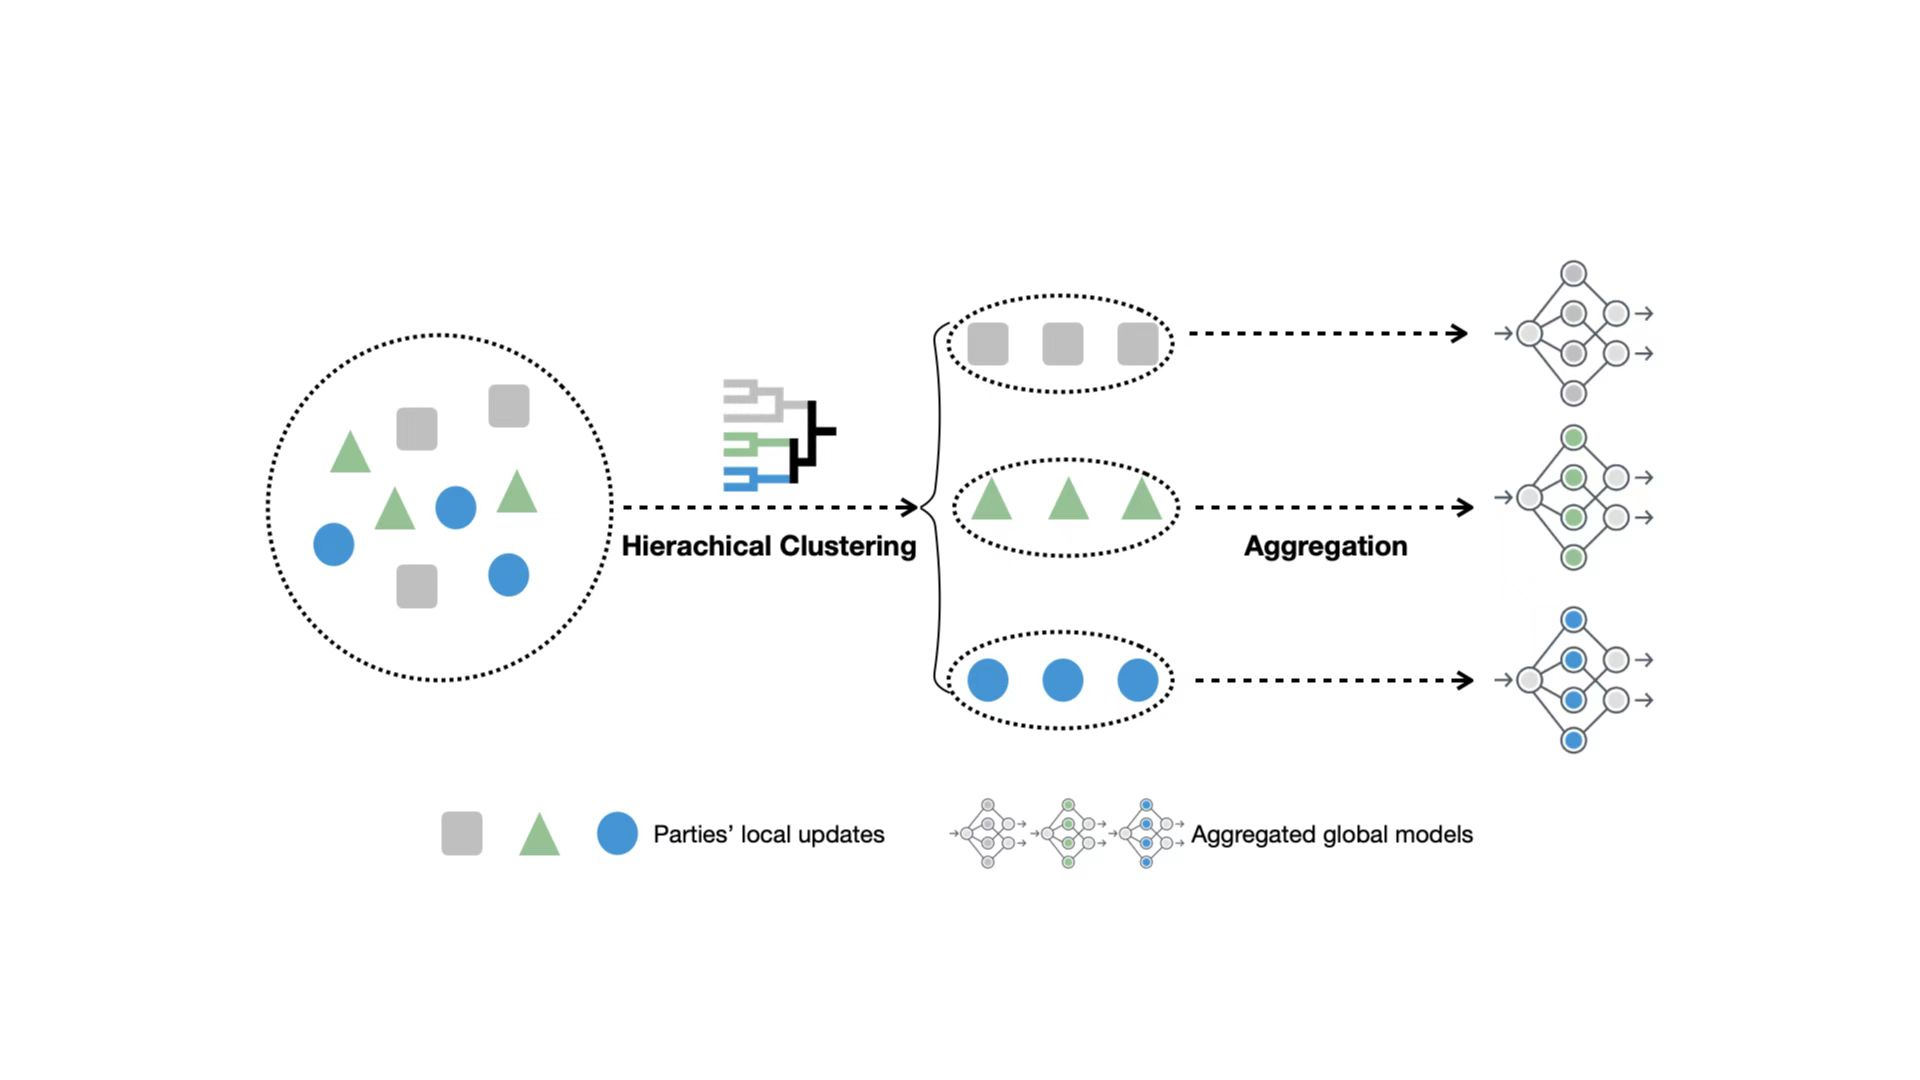
\includegraphics[scale=0.13]{figures/work2figs/hc.jpg}
        \caption{FL+HC简介}
        \label{hcjpg}
    \end{center}
\end{figure}

\subsection{密码技术介绍}

\subsubsection{加性秘密共享}
加性秘密共享是Shamir \cite{shamir1979share} 提出的一种安全多方计算技术。本章我们使用的是一种(2,2)的加性秘密共享方案,可用于安全两方计算(2PC)。这种方案可以在不同大小的环上做两方的安全计算,本章使用到的是两种特殊的环,环$\mathbb{Z}_2$和$\mathbb{p}, p=2^l$($l$一般为32)。当使用环$\mathbb{Z}_2$时,也被称为布尔秘密共享。
在布尔秘密共享方案中,布尔值$x \in \mathbb{Z}_2$可以被拆分为布尔共享份$\langle x\rangle_0^B$ 和 $\langle x\rangle_1^B$,其中三者满足$x = \langle x\rangle_0^B \oplus \langle x\rangle_0^B\;\text{mod}\;2$。
在使用环$x \in \mathbb{Z}_p$时,可以把环$\mathbb{Z}_p$上的元素$x$拆分为两个共享份$(\langle x\rangle_0, \langle x\rangle_1) = (r, x -r) \in \mathbb{Z}_p^2$, 其中$r$是在环$\mathbb{Z}_p$上随机采样得到的元素。通过执行安全的两方计算协议 \cite{rathee2020cryptflow2, rathee2021sirnn},在不重构出原始值的情况下,完成任意的算术运算。

\subsubsection{本章使用的安全两方计算(2PC)协议}
为了在共享份额上进行进行安全的计算,我们使用到了三种加性秘密共享上的基本运算 \cite{rathee2021sirnn},其基本信息的描述如下:
\begin{compactitem}
    \item \textbf{安全两方有符号数乘法}(Signed Value Multiplication,$\mathcal{F}_{\text{SMul}}$): 有符号数乘法 $(\mathcal{F}_{\text{SMul}})$ 以两方上的共享份额 $\langle x\rangle$ 以及 $\langle y\rangle$ 作为输入,然后输出 $\langle z\rangle$,其中三者满足:$z = x \times y$。
    \item \textbf{安全两方多路选择器}(Multiplexer,$\mathcal{F}_{\text{MUX}}$): 多路选择器 $(\mathcal{F}_{\text{MUX}})$ 以 $\langle x\rangle^B$ 和 $\langle y\rangle$ 作为输入,然后输出 $\langle z\rangle$,其中如果$x = 1$,则输出的$z$满足$z = y$,否则满足$z = 0$。 
    \item \textbf{安全两方DRelu} $(\mathcal{F}_{\text{DRelu}})$: DRelu 函数 $(\mathcal{F}_{\text{DRelu}})$ 以 $\langle x\rangle$ 作为输入,然后输出 $\langle z\rangle^B$,其中如果$x \geq 0$,则输出的$z$满足 $z = 1$,否则满足 $z = 0$。
\end{compactitem}

\subsubsection{伪随机生成技术}
伪随机生成技术(Pseudorandom Generator, PRG)\cite{yao1982theory} 可以根据一个均匀分布的随机数种子,生成一串很长的伪随机字符。只要这个随机数种子不被敌对方窃取,就能保证生成的这段随机字符,无法在多项式时间内与均匀分布采样出来的字符串做出区分。本章方案使用伪随机生成技术在参数上传和分发阶段保证参数隐私的同时,减少一半的通信开销(细节见\ref{4-framework})。

\section{问题描述}\label{4-problem}
本节我们主要对本章设计的的面向异质数据的隐私梯度聚合方案的系统模型、威胁模型以及设计目标,进行展开描述。

\subsection{系统模型}
本章设计的的面向异质数据的隐私保护梯度聚合方案系统模型如图\ref{sysjpg}所示。图中有$n$个参与方$P_1,P_2,...,P_n$和两个不共谋的服务器(FL服务提供商(SP)和计算服务器(CS)),这种实体分布在相似的研究\cite{liu2021privacy, dong2021flod, hao2021efficient}中非常常见。SP主导整个联合学习过程,而CS在必要的时机协助SP完成秘密共享份额上的安全两方计算(2PC),每个参与方$P$拥有用于联合训练的本地数据集$D$(用户间的数据分布时异质的),每个参与方的目标是联合与其有着同样学习目标的其他参与方(即数据分布一致),联合训练得到性能更好的全局模型。本章方案主要有以下三个步骤:
\begin{compactenum}
    \item SP将本轮全局模型广播给对应的用户。
    \item 每个参与方$P$将收到的全局模型应用到本地,然后利用本地数据$D$来更新模型参数,最后将更新梯度加密后发送给SP。
    \item 最后SP联合CS进行根据层次聚类结果,利用2PC协议进行安全的梯度聚合。
\end{compactenum}


\begin{figure}[htbp]
    \begin{center}
        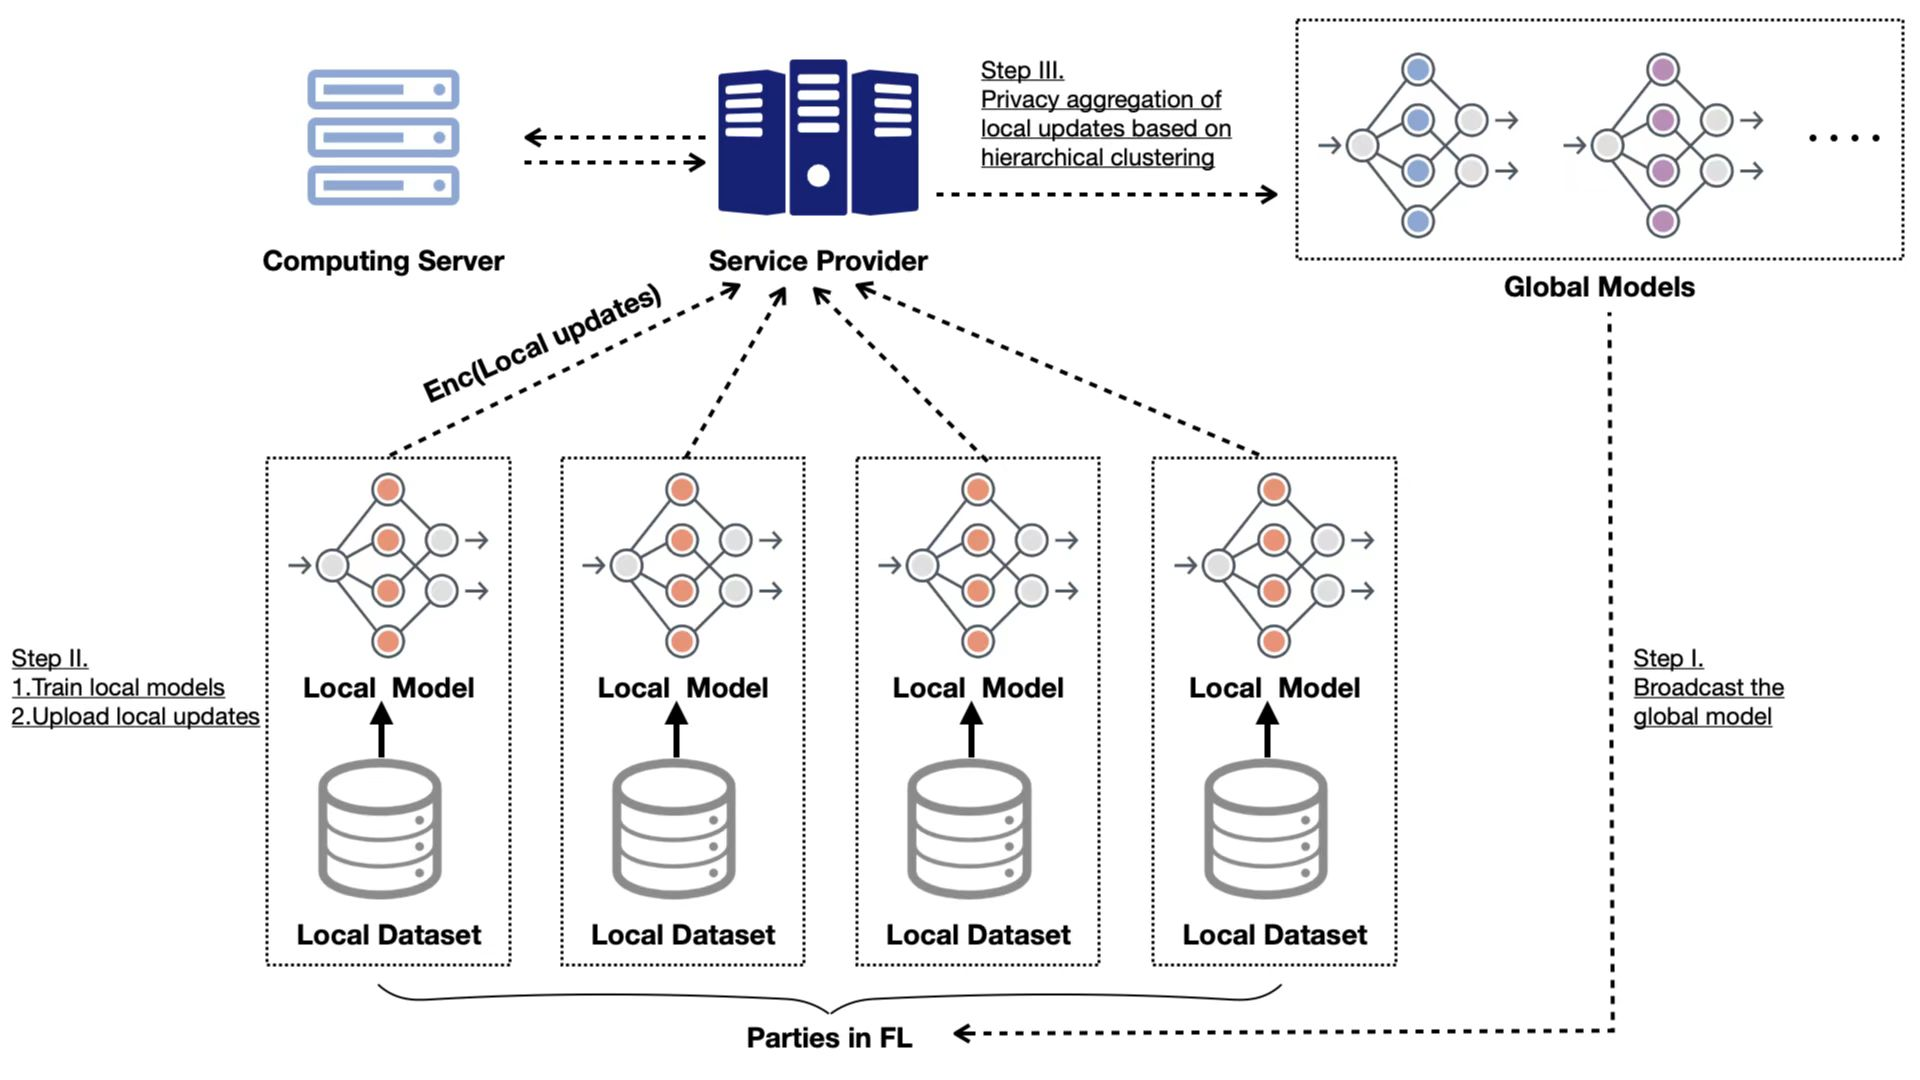
\includegraphics[scale=0.13]{figures/work2figs/system-model.jpg}
        \caption{PPFL+HC系统模型图}
        \label{sysjpg}
    \end{center}
\end{figure}

\subsection{威胁模型}
在本章方案中,我们将服务器(SP和CS)视为诚实且好奇的,这意味着SP和CS将严格执行我们设计的安全协议,但是会主动的尝试推断用户的隐私信息。除此之外,我们还假设,SP和CS因为害怕公信力的丧失,不会发生共谋行为,这可以保证我们按照(2,2)加性秘密共享上传的用户梯度不会泄露给服务器。这个威胁模型是可以在真实世界满足的,并且在类似工作\cite{nguyen2022flame}中也用到了同样的威胁模型。比如说,Google和Amazon两种服务提供商,为了维护自己的信誉,都会选择正确执行我们设计的安全协议,而不是共谋获取用户的隐私信息。

\subsection{设计目标}
本章的目标是在保证用户梯度隐私的同时,提升FL在面对异质数据的联合训练性能。具体来说,我们的设计目标如下:
\begin{compactitem}
    \item \textbf{梯度隐私保护:}我们致力于实现对梯度的完全隐私保护,其中包括对用户上传的本地梯度的隐私保护,以及聚合之后的全局梯度的隐私保护。
    \item \textbf{异质数据准确率提升:}我们通过实现对梯度共享份上的安全层次聚类,来提升FL在面对异质数据的联合训练性能下降问题。
    \item \textbf{高效的安全计算协议:}我们精心设计了2PC协议,保证在聚类以及聚合结果正确性的同时,尽量减小计算和通信的复杂度。
\end{compactitem}

\section{基于秘密共享的隐私保护计算模块}\label{4-building}
%介绍为什么要设计这几个模块
为了对$n$个参与方的梯度向量的共享份$\{\boldsymbol{\langle g_1\rangle}, \boldsymbol{\langle g_2\rangle},...,\boldsymbol{\langle g_n\rangle} \}$进行安全的层次聚类操作,最首要的工作就是度量梯度向量之间的相似性,在层次聚类中,度量方式有欧式距离、曼哈顿距离以及余弦相似度,鉴于余弦相似度计算涉及到的开方和除法在共享份上的计算开销较大,本章仅考虑安全的欧式距离计算和安全的曼哈顿距离计算,最后提出了基于安全距离度量的安全层次聚类算法。

\subsection{安全欧式距离计算}
为了安全的计算共享梯度向量$\boldsymbol{\langle g_i\rangle}$和$\boldsymbol{\langle g_j\rangle}$之间的欧式距离$\Vert \boldsymbol{g_i} - \boldsymbol{g_j} \Vert_2$,我们设计了安全的欧式距离(Secure Euclidean Distance, SED)计算算法。
首先SP和CS在本地计算$\boldsymbol{\langle z\rangle} = \boldsymbol{\langle g_i\rangle} - \boldsymbol{\langle g_j\rangle}$,然后SP和CS对于两个向量中的每一个元素协同调用$\mathcal{F}_{\text {SMul}}$,其中SP的输i入是$\boldsymbol{\langle z\rangle_0}[i]$,CS的输入是$\boldsymbol{\langle z\rangle_1}[i]$,然后SP和CS得到乘法的计算结果的共享份$\boldsymbol{\langle d\rangle}[i]$。
接下来SP和CS在本地计算向量$\boldsymbol{\langle d\rangle}$所有元素的内部和$\sum_{i=1}^{m} \boldsymbol{\langle d\rangle}[i]$,得到欧式距离平方的共享份$\langle \textit{EDis}^2\rangle$。
最后CS将共享份额$\langle \textit{EDis}^2\rangle_1$发送给SP,SP完成重构得到欧式距离明文$\textit{EDis}$(我们认为这个解密行为不会侵犯用户隐私,具体见安全性分析\ref{4-analysis})。
通过运行SED,SP和CS可以在不泄漏$\boldsymbol{g_i}$和$\boldsymbol{g_j}$每一个元素的情况下,得到梯度之间的欧式距离$\textit{EDis}$。SED算法的细节描述如算法\ref{alg1}所示。

\begin{algorithm}[htbp]
    \caption{安全欧式距离计算\\$\text{SED}(\boldsymbol{\langle g_i\rangle}, \boldsymbol{\langle g_j\rangle}) \xrightarrow{} \textit{EDis}$}
    \label{alg1}
    % \renewcommand{\algorithmicrequire}{\textbf{Input:}}
    % \renewcommand{\algorithmicensure}{\textbf{Output:}}
    \begin{algorithmic}[1]
    \REQUIRE SP拥有$\boldsymbol{\langle g_i\rangle_0}$和$\boldsymbol{\langle g_j\rangle_0}$, CS拥有$\boldsymbol{\langle g_i\rangle_1}$和$\boldsymbol{\langle g_j\rangle_1}$。 $\mathcal{F}_{\text {SMul}}$在文献\cite{rathee2021sirnn}中提出。
    \ENSURE $\boldsymbol{g_i}$和$\boldsymbol{g_j}$之间的欧式距离$\textit{EDis}$。
    % content
    \STATE SP本地计算$\boldsymbol{\langle z\rangle_0} = \boldsymbol{\langle g_i\rangle_0} - \boldsymbol{\langle g_j\rangle_0}$
    \STATE CS本地计算$\boldsymbol{\langle z\rangle_1} = \boldsymbol{\langle g_i\rangle_1} - \boldsymbol{\langle g_j\rangle_1}$
    % \STATE $\mathcal{F}_{\text {SMul }}(\langle z\rangle, \langle z\rangle)$
%    \FOR[$m$是$\boldsymbol{g_i}$的维度]{$i \in 1\:\textbf{to}\:m$} %\COMMENT{$m$ is the dimension of $\boldsymbol{g_i}$}
%        \STATE SP和CS调用函数$\mathcal{F}_{\text {SMul}}$, 其中SP的输入是$\boldsymbol{\langle z\rangle_0}[i]$,而CS的输入是 $\boldsymbol{\langle z\rangle_1}[i]$. 运算结束后SP和CS分别得到乘法结果的共享份$\boldsymbol{\langle d\rangle_0}[i]$ 和 $\boldsymbol{\langle d\rangle_1}[i]$。
%        % \STATE $(\lrangle EDis[i]\rangle,angle EDis[i]\rangle = \mathcal{F}_{\text {SMul }}(\langle z\rangle[i], \langle z\rangle[i])$
%    \ENDFOR
    \STATE SP和CS调用函数$\mathcal{F}_{\text {SMul}}$,其中输入为SP和CS持有的共享份$\boldsymbol{\langle z\rangle}$,计算得到乘法结果的共享份$\boldsymbol{\langle d\rangle}$ \COMMENT{对向量$\boldsymbol{\langle z\rangle}$中的元素逐个调用$\mathcal{F}_{\text {SMul}}$}
    \STATE SP本地计算$\langle \textit{EDis}^2\rangle_0 = \sum_{i=1}^{m} \boldsymbol{\langle d\rangle_0}[i]$
    \STATE CS本地计算$\langle \textit{EDis}^2\rangle_1 = \sum_{i=1}^{m} \boldsymbol{\langle d\rangle_1}[i]$
    \STATE CS发送$\langle \textit{EDis}^2\rangle_1$给SP, SP重构$\textit{EDis}^2 = \langle \textit{EDis}^2\rangle_0 + \langle \textit{EDis}^2\rangle_1$然后开方得到$\textit{EDis}$。
    \RETURN SP得到欧氏距离$\textit{EDis}$。
    \end{algorithmic}
\end{algorithm}

\subsection{安全曼哈顿距离计算}
为了安全的计算共享梯度向量$\boldsymbol{\langle g_i\rangle}$和$\boldsymbol{\langle g_j\rangle}$之间的曼哈顿距离$\norm{\boldsymbol{g_i} - \boldsymbol{g_j}}_1$,我们设计了安全的曼哈顿距离(Secure Manhattan Distance, SMD)计算算法。
首先SP和CS在本地计算$\boldsymbol{\langle z\rangle} = \boldsymbol{\langle g_i\rangle} - \boldsymbol{\langle g_j\rangle}$,然后SP联合CS以共享份$\boldsymbol{\langle z\rangle}$为输入,调用函数$\mathcal{F}_{\text {SMul}}$,计算得到DRelu值的布尔共享份$\boldsymbol{\langle y\rangle}^{B}$。
接着SP和CS分别计算$\boldsymbol{\langle \widetilde{y} \rangle_0}^{B} = \boldsymbol{\langle y\rangle_0}^{B}$和$\boldsymbol{\langle \widetilde{y} \rangle_1}^{B} = \boldsymbol{\langle y\rangle_1}^{B} \oplus 1$,得到DRelu结果对应的布尔取反结果$\boldsymbol{\langle \widetilde{y} \rangle}^{B}$。
紧接着SP和CS调用两次安全多路选择器,分别以$\{\boldsymbol{\langle z\rangle}, \boldsymbol{\langle y\rangle}^{B}\}$、$\{\boldsymbol{\langle z\rangle}, \boldsymbol{\langle \widetilde{y}\rangle}^{B}\}$为输入,获取$\boldsymbol{\langle z\rangle}$中的正数集合$\boldsymbol{
	\langle d_p\rangle}$以及负数集合$\boldsymbol{
	\langle d_n\rangle}$。
最后SP和CS在本地计算$\langle \textit{MDis}\rangle = \sum_{i=1}^{m}\boldsymbol{\langle d_p\rangle}[i] - \sum_{i=1}^{m}\boldsymbol{\langle d_n\rangle}[i]$,CS将结果共享份$\langle \textit{MDis}\rangle_1$发送给SP,SP完成重构得到曼哈顿距离$\textit{MDis}$。
SMD具体的算法细节描述如算法\ref{alg2}所示。

\begin{algorithm}[htbp]
    \caption{安全曼哈顿距离计算\\$\text{SMD}(\boldsymbol{\langle g_i\rangle}, \boldsymbol{\langle g_j\rangle}) \xrightarrow{} \textit{MDis}$}
    \label{alg2}
    \begin{algorithmic}[1]
    % \renewcommand{\algorithmicrequire}{\textbf{Input:}}
    % \renewcommand{\algorithmicensure}{\textbf{Output:}}
    \REQUIRE SP 拥有 $\boldsymbol{\langle g_i\rangle_0}$ 和 $\boldsymbol{\langle g_j\rangle_0}$, CS 拥有 $\boldsymbol{\langle g_i\rangle_1}$ 和 $\boldsymbol{\langle g_j\rangle_1}$. $\mathcal{F}_{\text {DRelu}}$ 和 $\mathcal{F}_{\text {MUX}}$ 在文献\cite{rathee2021sirnn}中提出。
    \ENSURE $\boldsymbol{g_i}$ 与 $\boldsymbol{g_j}$之间的曼哈顿距离$\textit{MDis}$。
    % content
    \STATE SP 本地计算 $\boldsymbol{\langle z\rangle_0} = \boldsymbol{\langle g_i\rangle_0} - \boldsymbol{\langle g_j\rangle_0}$
    \STATE CS 本地计算 $\boldsymbol{\langle z\rangle_1} = \boldsymbol{\langle g_i\rangle_1} - \boldsymbol{\langle g_j\rangle_1}$
    \STATE SP 和 CS 调用 $\mathcal{F}_{\text{DRelu}}$,其中输入为SP和CS持有的共享份$\boldsymbol{\langle z\rangle}$,计算得到DRelu值的布尔共享份$\boldsymbol{\langle y\rangle}^{B}$。
    \STATE SP 和 CS 分别调用 $\boldsymbol{\langle \widetilde{y} \rangle_0}^{B} = \boldsymbol{\langle y\rangle_0}^{B}$ 和 $\boldsymbol{\langle \widetilde{y} \rangle_1}^{B} = \boldsymbol{\langle y\rangle_1}^{B} \oplus 1$。\COMMENT{安全的获得布尔共享份$\boldsymbol{\langle y\rangle}^{B}$的取反结果$\boldsymbol{\langle \widetilde{y} \rangle}^{B}$。}
    % \State SP sets $\boldsymbol{\langle \widetilde{g_i}\rangle_0}$ = - $\boldsymbol{\langle g_i\rangle_0}$ and $\boldsymbol{\langle \widetilde{g_j}\rangle_0}$ = - $\boldsymbol{\langle g_j\rangle_0}$
    % \State CS sets $\boldsymbol{\langle \widetilde{g_i}\rangle_1}$ = - $\boldsymbol{\langle g_i\rangle_1}$ and $\boldsymbol{\langle \widetilde{g_j}\rangle_1}$ = - $\boldsymbol{\langle g_j\rangle_1}$
    % \For{$i \in [1...m]$} \Comment{$m$ is the dimension of $\boldsymbol{g_i}$}
        \STATE SP 和 CS 调用 $\mathcal{F}_{\text{MUX}}$,其中输入为SP和CS持有的共享份$\boldsymbol{\langle z\rangle}$ 和 $\boldsymbol{\langle y\rangle}^{B}$,计算得到$\boldsymbol{\langle z\rangle}$中的正数集合$\boldsymbol{
        \langle d_p\rangle}$。
        \STATE SP 和 CS 调用 $\mathcal{F}_{\text{MUX}}$,其中输入为SP和CS持有的共享份 $\boldsymbol{\langle z\rangle}$ 和 $\boldsymbol{\langle \widetilde{y}\rangle}^{B}$,计算得到$\boldsymbol{\langle z\rangle}$中的负数集合$\boldsymbol{
        \langle d_n\rangle}$
    % \EndFor
    \STATE SP 本地计算 $\langle \textit{MDis}\rangle_0 = \sum_{i=1}^{m}\boldsymbol{\langle d_p\rangle_0}[i] - \sum_{i=1}^{m}\boldsymbol{\langle d_n\rangle_0}[i]$ \COMMENT{$m$ 是 $\boldsymbol{g_i}$的维度}
    \STATE CS 本地计算 $\langle \textit{MDis}\rangle_1 = \sum_{i=1}^{m}\boldsymbol{\langle d_p\rangle_1}[i] - \sum_{i=1}^{m}\boldsymbol{\langle d_n\rangle_1}[i]$
    \STATE CS 发送 $\langle \textit{MDis}\rangle_1$ 给 SP,然后SP 重构出 $\textit{MDis} = \langle \textit{MDis}\rangle_0 + \langle \textit{MDis}\rangle_1$。
    \RETURN SP得到曼哈顿距离$\textit{MDis}$。
    \end{algorithmic}
\end{algorithm}

\subsection{安全的梯度层次聚类}
%写随机梯度裁剪
为了完成对共享份梯度集合$\{\boldsymbol{\langle g_1\rangle}, \boldsymbol{\langle g_2\rangle},...,\boldsymbol{\langle g_n\rangle} \}$的安全层次聚类,我们将整个聚类过程划分为两个阶段:
\begin{compactenum}
	\item \textbf{梯度间距离矩阵计算:}这一阶段完成每个共享梯度向量$\svec{g_i}$,与其它$n-1$梯度的距离计算,得到一个距离矩阵$\{\textit{Dis}_{00}, \textit{Dis}_{01},...,\textit{Dis}_{nn}\}$,其中距离的计算过程以梯度共享份为输入,调用上述SED或SMD安全距离计算算法,在保证梯度隐私的前提下,得到明文的距离矩阵。
	\item \textbf{基于距离矩阵的聚类过程:}在得到预先计算好的距离矩阵之后,再搭配其它层次聚类参数,比如不同的簇间距离计算方式($avg, min\; or\; max$)以及距离阈值,完成对梯度的自底向上的层次聚类。
\end{compactenum}
具体的层次聚类算法细节如算法\ref{alg3}所示。

\begin{algorithm}[htbp]
	\caption{安全的梯度层次聚类算法}
	\label{alg3}
	\begin{algorithmic}[1]
		\REQUIRE SP 和 CS 拥有$\{\boldsymbol{\langle g_1\rangle}, \boldsymbol{\langle g_2\rangle},...,\boldsymbol{\langle g_n\rangle} \}$。 \COMMENT{$n$ 是参与方数量}
		\ENSURE $l$ 个簇 $\{c_1,c_2,...,c_l \}$。
		% content
		\FOR{$i \gets 1\:\textbf{to}\:n$}
		\FOR{$j \gets 1\:\textbf{to}\:n$}
			\STATE SP 和 CS 调用$\textit{Dis}_{ij} \xleftarrow{}\text{SMD}\boldsymbol{\langle g_i\rangle}, \boldsymbol{\langle g_j\rangle})$ (或者 $\text{SED}\boldsymbol{\langle g_i\rangle}, \boldsymbol{\langle g_j\rangle})$), 然后SP获得距离值$\textit{Dis}_{ij}$。
		\ENDFOR
		\ENDFOR
		\STATE $\{c_1,c_2,...,c_l \} \xleftarrow{} \textsc{Clustering}(\textit{Dis}_{11},...,\textit{Dis}_{nn})$ \COMMENT{基于预计算距离矩阵的层次聚类}
		\RETURN SP和CS获得层次聚类结果 $\{c_1,c_2,...,c_l \}$。
	\end{algorithmic}
\end{algorithm}



\section{面向异质数据的隐私保护梯度聚合方案}\label{4-framework}

%option
\section{安全性分析}\label{4-analysis}

\section{实验评估}\label{4-exp}

\section{本章小结}\label{4-conclusion}